\documentclass[journal,12pt,twocolumn]{IEEEtran}
%
\usepackage{setspace}
\usepackage{gensymb}
\usepackage{xcolor}
\usepackage{caption}
%\usepackage{subcaption}
%\doublespacing
\singlespacing

%\usepackage{graphicx}
%\usepackage{amssymb}
%\usepackage{relsize}
\usepackage[cmex10]{amsmath}
\usepackage{mathtools}
%\usepackage{amsthm}
%\interdisplaylinepenalty=2500
%\savesymbol{iint}
%\usepackage{txfonts}
%\restoresymbol{TXF}{iint}
%\usepackage{wasysym}
\usepackage{amsthm}
\usepackage{mathrsfs}
\usepackage{txfonts}
\usepackage{stfloats}
\usepackage{cite}
\usepackage{cases}
\usepackage{subfig}
%\usepackage{xtab}
\usepackage{longtable}
\usepackage{multirow}
%\usepackage{algorithm}
%\usepackage{algpseudocode}
\usepackage{enumitem}
\usepackage{mathtools}
%\usepackage{iithtlc}
%\usepackage[framemethod=tikz]{mdframed}
\usepackage{listings}
\usepackage{listings}
    \usepackage[latin1]{inputenc}                                 %%
    \usepackage{color}                                            %%
    \usepackage{array}                                            %%
    \usepackage{longtable}                                        %%
    \usepackage{calc}                                             %%
    \usepackage{multirow}                                         %%
    \usepackage{hhline}                                           %%
    \usepackage{ifthen}                                           %%
  %optionally (for landscape tables embedded in another document): %%
    \usepackage{lscape}     



%\usepackage{stmaryrd}


%\usepackage{wasysym}
%\newcounter{MYtempeqncnt}
\DeclareMathOperator*{\Res}{Res}
%\renewcommand{\baselinestretch}{2}
\renewcommand\thesection{\arabic{section}}
\renewcommand\thesubsection{\thesection.\arabic{subsection}}
\renewcommand\thesubsubsection{\thesubsection.\arabic{subsubsection}}

\renewcommand\thesectiondis{\arabic{section}}
\renewcommand\thesubsectiondis{\thesectiondis.\arabic{subsection}}
\renewcommand\thesubsubsectiondis{\thesubsectiondis.\arabic{subsubsection}}

% correct bad hyphenation here
\hyphenation{op-tical net-works semi-conduc-tor}

\lstset{
language=C,
frame=single, 
breaklines=true
}

%\lstset{
	%%basicstyle=\small\ttfamily\bfseries,
	%%numberstyle=\small\ttfamily,
	%language=Octave,
	%backgroundcolor=\color{white},
	%%frame=single,
	%%keywordstyle=\bfseries,
	%%breaklines=true,
	%%showstringspaces=false,
	%%xleftmargin=-10mm,
	%%aboveskip=-1mm,
	%%belowskip=0mm
%}

%\surroundwithmdframed[width=\columnwidth]{lstlisting}
\def\inputGnumericTable{}                                 %%
\lstset{
language=C,
frame=single, 
breaklines=true
}
 

\begin{document}
%

\theoremstyle{definition}
\newtheorem{theorem}{Theorem}[section]
\newtheorem{problem}{Problem}
\newtheorem{proposition}{Proposition}[section]
\newtheorem{lemma}{Lemma}[section]
\newtheorem{corollary}[theorem]{Corollary}
\newtheorem{example}{Example}[section]
\newtheorem{definition}{Definition}[section]
%\newtheorem{algorithm}{Algorithm}[section]
%\newtheorem{cor}{Corollary}
\newcommand{\BEQA}{\begin{eqnarray}}
\newcommand{\EEQA}{\end{eqnarray}}
\newcommand{\define}{\stackrel{\triangle}{=}}

\bibliographystyle{IEEEtran}
%\bibliographystyle{ieeetr}

\providecommand{\nCr}[2]{\,^{#1}C_{#2}} % nCr
\providecommand{\nPr}[2]{\,^{#1}P_{#2}} % nPr
\providecommand{\mbf}{\mathbf}
\providecommand{\pr}[1]{\ensuremath{\Pr\left(#1\right)}}
\providecommand{\qfunc}[1]{\ensuremath{Q\left(#1\right)}}
\providecommand{\sbrak}[1]{\ensuremath{{}\left[#1\right]}}
\providecommand{\lsbrak}[1]{\ensuremath{{}\left[#1\right.}}
\providecommand{\rsbrak}[1]{\ensuremath{{}\left.#1\right]}}
\providecommand{\brak}[1]{\ensuremath{\left(#1\right)}}
\providecommand{\lbrak}[1]{\ensuremath{\left(#1\right.}}
\providecommand{\rbrak}[1]{\ensuremath{\left.#1\right)}}
\providecommand{\cbrak}[1]{\ensuremath{\left\{#1\right\}}}
\providecommand{\lcbrak}[1]{\ensuremath{\left\{#1\right.}}
\providecommand{\rcbrak}[1]{\ensuremath{\left.#1\right\}}}
\theoremstyle{remark}
\newtheorem{rem}{Remark}
\newcommand{\sgn}{\mathop{\mathrm{sgn}}}
\providecommand{\abs}[1]{\left\vert#1\right\vert}
\providecommand{\res}[1]{\Res\displaylimits_{#1}} 
\providecommand{\norm}[1]{\lVert#1\rVert}
\providecommand{\mtx}[1]{\mathbf{#1}}
\providecommand{\mean}[1]{E\left[ #1 \right]}
\providecommand{\fourier}{\overset{\mathcal{F}}{ \rightleftharpoons}}
%\providecommand{\hilbert}{\overset{\mathcal{H}}{ \rightleftharpoons}}
\providecommand{\system}{\overset{\mathcal{H}}{ \longleftrightarrow}}
	%\newcommand{\solution}[2]{\textbf{Solution:}{#1}}
\newcommand{\solution}{\noindent \textbf{Solution: }}
\providecommand{\dec}[2]{\ensuremath{\overset{#1}{\underset{#2}{\gtrless}}}}
%\numberwithin{equation}{subsection}
\numberwithin{equation}{problem}
%\numberwithin{problem}{subsection}
%\numberwithin{definition}{subsection}
\makeatletter
\@addtoreset{figure}{problem}
\makeatother

\let\StandardTheFigure\thefigure
%\renewcommand{\thefigure}{\theproblem.\arabic{figure}}
\renewcommand{\thefigure}{\theproblem}


%\numberwithin{figure}{subsection}

%\numberwithin{equation}{subsection}
%\numberwithin{equation}{section}
%%\numberwithin{equation}{problem}
%%\numberwithin{problem}{subsection}
%\numberwithin{problem}{section}
%%\numberwithin{definition}{subsection}
%\makeatletter
%\@addtoreset{figure}{problem}
%\makeatother
%\makeatletter
%\@addtoreset{table}{problem}
%\makeatother

%\let\StandardTheFigure\thefigure
%\let\StandardTheTable\thetable
%%\renewcommand{\thefigure}{\theproblem.\arabic{figure}}
%\renewcommand{\thefigure}{\theproblem}
%\renewcommand{\thetable}{\theproblem}
%%\numberwithin{figure}{section}

%%\numberwithin{figure}{subsection}



\def\putbox#1#2#3{\makebox[0in][l]{\makebox[#1][l]{}\raisebox{\baselineskip}[0in][0in]{\raisebox{#2}[0in][0in]{#3}}}}
     \def\rightbox#1{\makebox[0in][r]{#1}}
     \def\centbox#1{\makebox[0in]{#1}}
     \def\topbox#1{\raisebox{-\baselineskip}[0in][0in]{#1}}
     \def\midbox#1{\raisebox{-0.5\baselineskip}[0in][0in]{#1}}

\vspace{3cm}

\title{ Bluetooth Based IOT through Arduino
	%\logo{Introduction to Math Computing 
	%}
}
%\title{
%	\logo{Matrix Analysis through Octave}{\begin{center}\includegraphics[scale=.24]{tlc}\end{center}}{}{HAMDSP}
%}


% paper title
% can use linebreaks \\ within to get better formatting as desired
%\title{Matrix Analysis through Octave}
%
%
% author names and IEEE memberships
% note positions of commas and nonbreaking spaces ( ~ ) LaTeX will not break
% a structure at a ~ so this keeps an author's name from being broken across
% two lines.
% use \thanks{} to gain access to the first footnote area
% a separate \thanks must be used for each paragraph as LaTeX2e's \thanks
% was not built to handle multiple paragraphs
%

\author{G V V Sharma$^{*}$ %<-this  stops a space
\thanks{*The author is with the Department
of Electrical Engineering, Indian Institute of Technology, Hyderabad
502285 India e-mail:  gadepall@iith.ac.in.}% <-this % stops a space
%\thanks{J. Doe and J. Doe are with Anonymous University.}% <-this % stops a space
%\thanks{Manuscript received April 19, 2005; revised January 11, 2007.}}
}
% note the % following the last \IEEEmembership and also \thanks - 
% these prevent an unwanted space from occurring between the last author name
% and the end of the author line. i.e., if you had this:
% 
% \author{....lastname \thanks{...} \thanks{...} }
%                     ^------------^------------^----Do not want these spaces!
%
% a space would be appended to the last name and could cause every name on that
% line to be shifted left slightly. This is one of those "LaTeX things". For
% instance, "\textbf{A} \textbf{B}" will typeset as "A B" not "AB". To get
% "AB" then you have to do: "\textbf{A}\textbf{B}"
% \thanks is no different in this regard, so shield the last } of each \thanks
% that ends a line with a % and do not let a space in before the next \thanks.
% Spaces after \IEEEmembership other than the last one are OK (and needed) as
% you are supposed to have spaces between the names. For what it is worth,
% this is a minor point as most people would not even notice if the said evil
% space somehow managed to creep in.



% The paper headers
%\markboth{Journal of \LaTeX\ Class Files,~Vol.~6, No.~1, January~2007}%
%{Shell \MakeLowercase{\textit{et al.}}: Bare Demo of IEEEtran.cls for Journals}
% The only time the second header will appear is for the odd numbered pages
% after the title page when using the twoside option.
% 
% *** Note that you probably will NOT want to include the author's ***
% *** name in the headers of peer review papers.                   ***
% You can use \ifCLASSOPTIONpeerreview for conditional compilation here if
% you desire.




% If you want to put a publisher's ID mark on the page you can do it like
% this:
%\IEEEpubid{0000--0000/00\$00.00~\copyright~2007 IEEE}
% Remember, if you use this you must call \IEEEpubidadjcol in the second
% column for its text to clear the IEEEpubid mark.



% make the title area
\maketitle

%\newpage

%\tableofcontents


%\begin{abstract}
%%\boldmath
%In this letter, an algorithm for evaluating the exact analytical bit error rate  (BER)  for the piecewise linear (PL) combiner for  multiple relays is presented. Previous results were available only for upto three relays. The algorithm is unique in the sense that  the actual mathematical expressions, that are prohibitively large, need not be explicitly obtained. The diversity gain due to multiple relays is shown through plots of the analytical BER, well supported by simulations. 
%
%\end{abstract}
% IEEEtran.cls defaults to using nonbold math in the Abstract.
% This preserves the distinction between vectors and scalars. However,
% if the journal you are submitting to favors bold math in the abstract,
% then you can use LaTeX's standard command \boldmath at the very start
% of the abstract to achieve this. Many IEEE journals frown on math
% in the abstract anyway.

% Note that keywords are not normally used for peerreview papers.
%\begin{IEEEkeywords}
%Cooperative diversity, decode and forward, piecewise linear
%\end{IEEEkeywords}



% For peer review papers, you can put extra information on the cover
% page as needed:
% \ifCLASSOPTIONpeerreview
% \begin{center} \bfseries EDICS Category: 3-BBND \end{center}
% \fi
%
% For peerreview papers, this IEEEtran command inserts a page break and
% creates the second title. It will be ignored for other modes.
\IEEEpeerreviewmaketitle


%\documentclass{article}
%\usepackage[utf8]{inputenc}
%\usepackage{listings}
%\usepackage{graphicx}

%\usepackage{color}
%\definecolor{codegreen}{rgb}{0,0.6,0}
%\definecolor{codegray}{rgb}{0.5,0.5,0.5}
%\definecolor{codepurple}{rgb}{0.58,0,0.82}
%\definecolor{backcolour}{rgb}{0.95,0.95,0.92}
%\lstdefinestyle{mystyle}{
    %backgroundcolor=\color{backcolour},   
    %commentstyle=\color{codegreen},
    %keywordstyle=\color{magenta},
    %numberstyle=\tiny\color{codegray},
    %stringstyle=\color{codepurple},
    %basicstyle=\footnotesize,
    %breakatwhitespace=false,         
    %breaklines=true,                 
    %captionpos=b,                    
    %keepspaces=true,                 
    %numbers=left,                    
    %numbersep=5pt,                  
    %showspaces=false,                
    %showstringspaces=false,
    %showtabs=false,                  
    %tabsize=2
%}
 
%\lstset{style=mystyle}


%\title{Analog Design Through Arduino}
%\author{G V V Sharma* }

%\begin{document}

%\maketitle
\section{Measuring the resistance}
\begin{problem}
Connect the 5V pin of the Arduino to an extreme pin of the Breadboard shown in Fig. \ref{fig:breadboard}.  Let this pin be $V_{cc}$.
\end{problem}
%
%
\begin{figure}
\centering
\includegraphics[width=\columnwidth]{./figs/breadboard.eps}
\caption{Breadboard}
\label{fig:breadboard}
\end{figure}
%
\begin{problem}
Connect the GND pin of the Arduino to the opposite extreme pin of the Breadboard.
\end{problem}
%
%
\begin{problem}
Let $R_1$ be the known resistor and $R_2$ be the unknown resistor.  Connect $R_1$ and $R_2$ in series such that $R_1$ is connected
to GND and $R_2$ is connected to $V_{cc}$. Refer to Fig. \ref{fig:voltage_divider}
\end{problem}
%
%
\begin{figure}
\centering
\includegraphics[width=\columnwidth]{./figs/voltage_divider.eps}
\caption{Voltage Divider}
\label{fig:voltage_divider}
\end{figure}
%

\begin{problem}
Connect the junction between the two resistors to  the A0 pin on the Arduino.
\end{problem}
%
\begin{problem}
Connect the arduino to the computer so that it is powered.
\end{problem}
%
\begin{problem}
Open the Arduino IDE and type the following code.  Open the {\em serial monitor} to view the output.
\end{problem}
%
\lstinputlisting{./codes/resistance/resistance.ino}
%
\section{Development of Android Application to Display the Measured Resistance via Bluetooth}
In the following, we make an android application using MIT App Inventor or Android studio (here we are using MIT App Inventor) to display the measured resistance. 

%
\begin{problem}
Click on link \textcolor{red}{http://appinventor.mit.edu/} for using MIT App Inventor.
\end{problem}
%
\begin{problem}
Click on \textcolor{red}{Create apps!} tag to get started.
\end{problem}
%
\includegraphics[width=\columnwidth]{./figs/1.png.eps}
%\includegraphics[height=8cm, width=16.6cm]{./figs/1.png.eps}
\begin{problem}
Log in to App Inventor with a gmail user name and password.
\end{problem}
%
\begin{problem}
Start a new project. Type in the project name (underscores are allowed, spaces are not) and click OK
\end{problem}
%
\begin{problem}
You are now in the Designer editor, where you lay out the "user interface" of your app
\end{problem}
%
\includegraphics[width=\columnwidth]{./figs/2.png.eps}
\begin{problem}
Click on "Layout" in the palette section. Then, click and hold on "HorizontalArrangement" and drag your mouse over to the Viewer. Drop the HorizontalArrangement and a new HorizontalArrangement will appear on the Viewer. This HorizontalArrangement is just to leave some blank space before placing something else for making the layout effective. Go to the properties of this HorizontalArrangement. Change the Height property to 10 percent and Width to "Fill parent". You can change the properties according to your requirement
\end{problem}
%
\includegraphics[width=\columnwidth]{./figs/7.png.eps}
\begin{problem}
Drag another HorizontalArrangement component onto the Viewer and change the Width property to ``Fill parent". From the User Interface component group, select and drag the ``ListPicker" component onto the 2nd HorizontalArrangement on Viewer. The ListPicker component provide similar function as Button that function like menu options, where you can click on one of the selection to get to the specified option.  Remove the text from the Text property of ListPicker and change the  AlignHorizontal property of HorizontalArrangement to ``Center". Download a .PNG bluetooth icon from the net.  Upload this image in the Image property of ListPicker for the symbol of bluetooth.  After uploading, change the Width and Height property of the ListPicker to 70 pixels. You won't see any bluetooth icon now.  Wait.
\end{problem}
%
\includegraphics[width=\columnwidth]{./figs/8.png.eps}
\begin{problem}
Drag another HorizontalArrangement component onto the Viewer and change the Width property to ``Fill parent". From the User Interface component group, select and drag the ``Label" component onto the 3rd HorizontalArrangement on Viewer. Change the Text property of Label to \textcolor{red}{Not Connected}. Change the  AlignHorizontal property of HorizontalArrangement to ``Center".
\end{problem}
%
\begin{problem}
Again drag a HorizontalArrangement component onto the Viewer. Change the Width property to ``Fill parent" and Height to 8 percent. This 4th HorizontalArrangement is also to leave some blank space before placing something else.
\end{problem}
%
\begin{problem}
Drag 5th HorizontalArrangement component onto the Viewer.Change the Height property to 15 percent and Width to "Fill parent". From the User Interface component group, select and drag the 2nd  "Label" component onto the 5th HorizontalArrangement on Viewer. Change the AlignHorizontal and AlignVertical property of  HorizontalArrangement to "Center". Remove the text from the Text property of Label and change the Width property to "Fill parent". Change the Text alignment property of Label to "Center" and Height to 5 percent.
\end{problem}
%
\begin{problem}
From the Connectivity component group in the Palette section, select and drag the BluetoothClient component to the Viewer. Since the BluetoothClient component does not have user interface, it is a non-visible component and not shown on the Viewer.
\end{problem}
%
\begin{problem}
Next, from the Sensors component group in the Palette section, select and drag the Clock component onto the Viewer. The Clock component is a non-visible component and does not shows up on the app screen. This is the user interface layout of the app.
\end{problem}
%
\includegraphics[width=\columnwidth]{./figs/3.png.eps}
\begin{problem}
Next, with all of the required layout components in place, click on the Blocks button to switch to the Block editor to add programming logic.
\end{problem}
%
\includegraphics[width=\columnwidth]{./figs/4.png.eps}
\begin{problem}
From the  Screen1$\backslash$ListPicker1 component group, select and add the ``when ListPicker1.BeforePicking" and ``set ListPicker1.Elements" components. From the  Screen1$\backslash$BluetooothClient1 component group, select and add the ``BluetoothClient1.AddressAndNames" component to the Viewer section. Assemble the blocks to get the following image.
\end{problem}
%
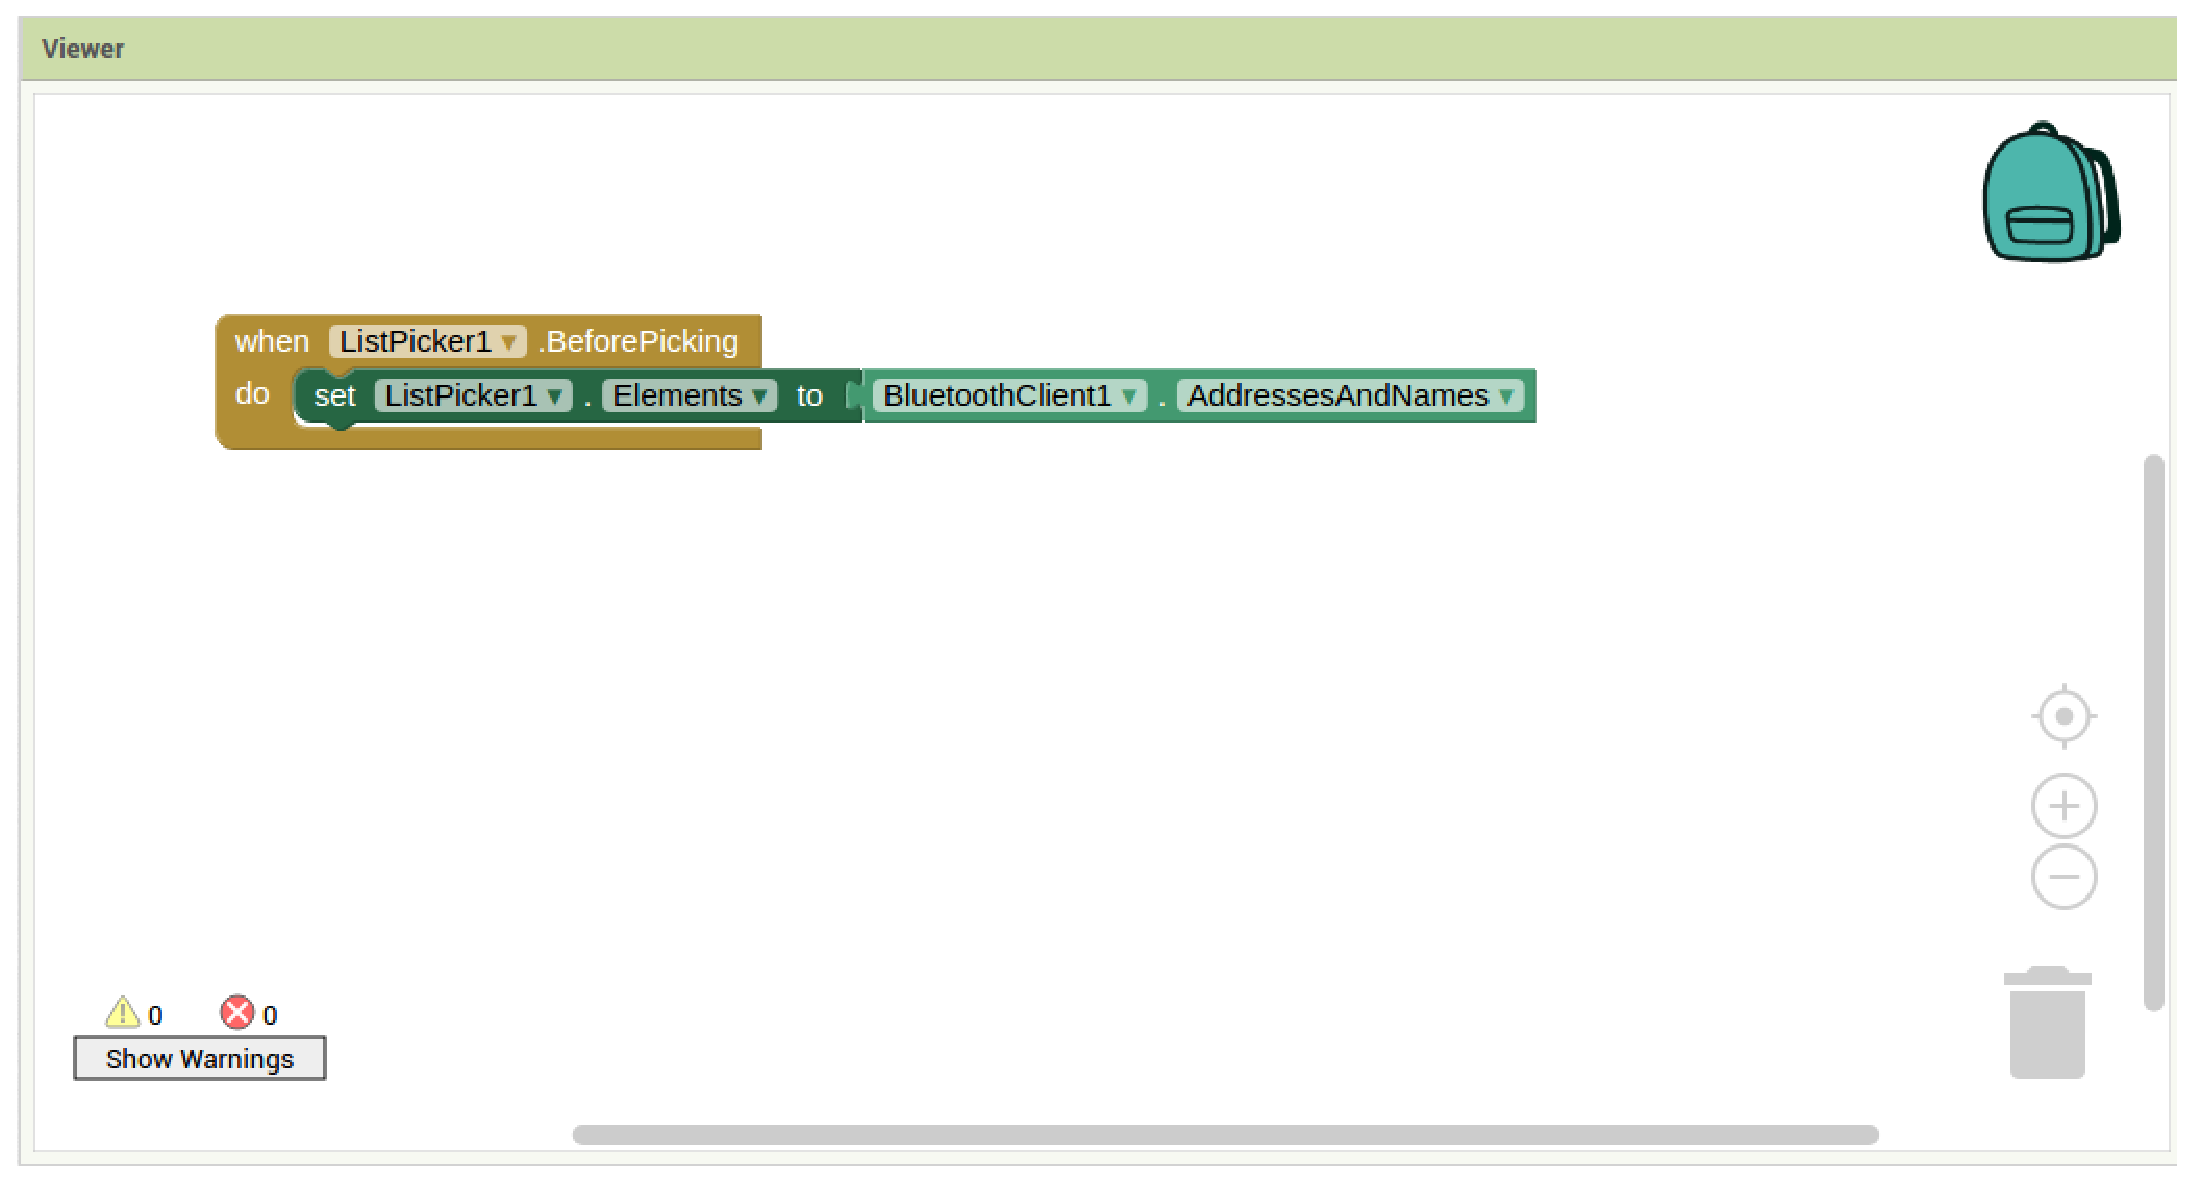
\includegraphics[width=\columnwidth]{./figs/9.png.eps}
\\
The above group of components provide the function to retrieve the list Bluetooth devices paired with the Android device.
\begin{problem}
Continue and add the ``when ListPicker1.AfterPicking" component from the  Screen1$\backslash$ListPicker1 component group to the Viewer section. The ListPicker1.AfterPicking component is an event handler after an item is selected. From the Built-in $\backslash$Control group, select and add the ``If then" component, a conditional handler, to the Viewer section.  
Next, select and add the ``call BluetoothClient1.Connect address" (from the Screen1$\backslash$BluetooothClient1 component group). and ``ListPicker1.Selection" (from the Screen1$\backslash$ListPicker1 component group) components and link to the ``if" condition. Again, from the Built-in $\backslash$Control group, select and add the ``If then" component and link to the ``then" condition. To extend the block with as many else and else if branches click the blue icon.  Do this to get the following image.
\end{problem}
%
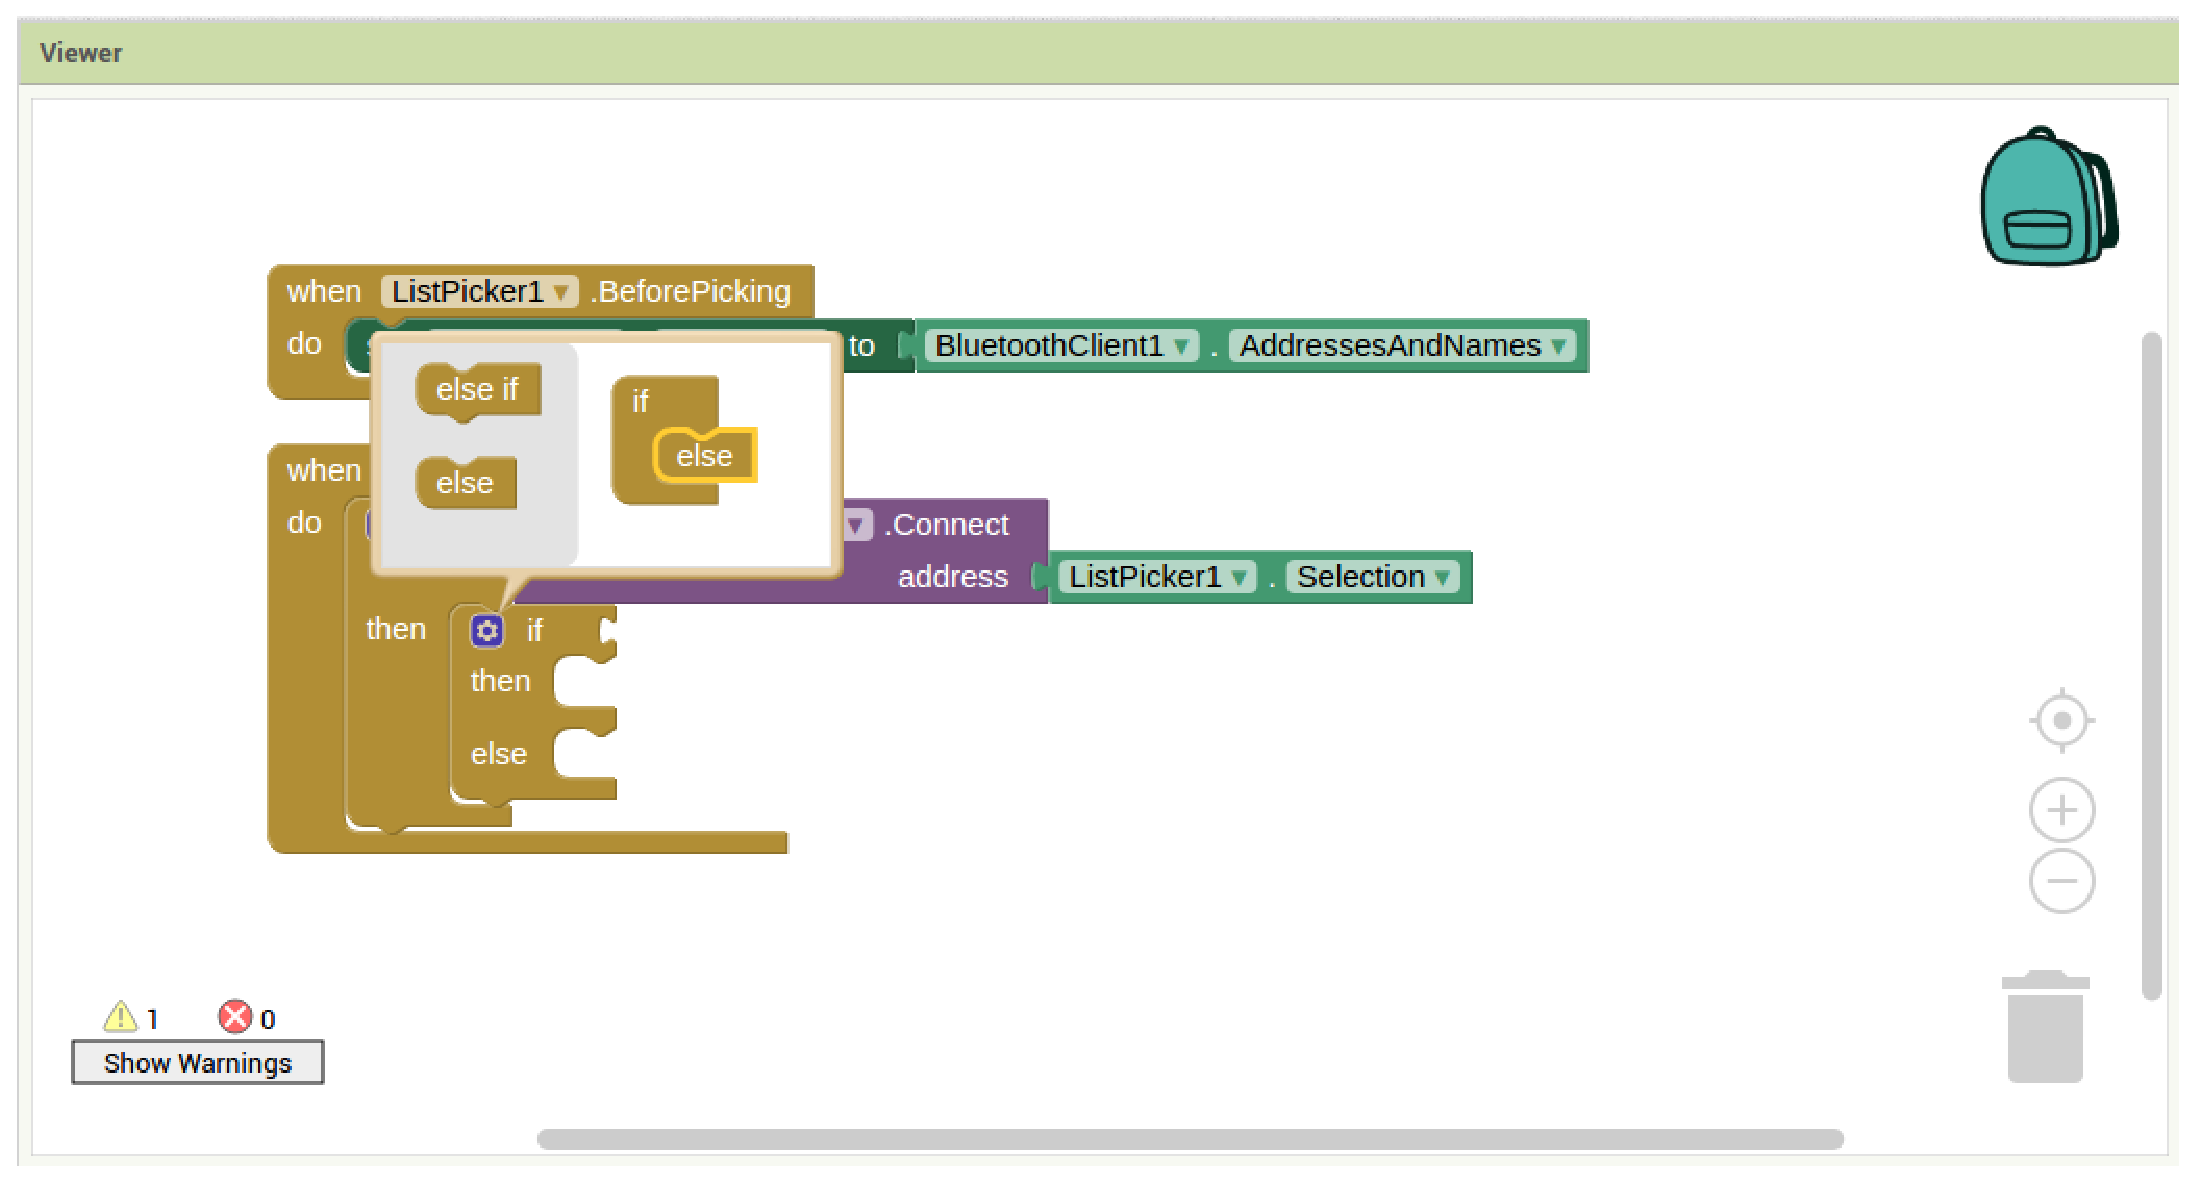
\includegraphics[width=\columnwidth]{./figs/10.png.eps}
\begin{problem}
Next, select and add the ``BluetoothClient1.IsConnected" (from the Screen1$\backslash$BluetooothClient1 component group) and link to the second ``if" condition. Select ``set Label1.Text" (from the Screen1$\backslash$Label1 component group) components and link to the ``then" condition and from the Built-in $\backslash$Text, click on the blank text entry component and enter the word \textcolor{green}{Connected}. Select ``set Label1.TextColor" (from the Screen1$\backslash$Label1 component group) components and link just below the ``Label1.Text" and from the Built-in $\backslash$Colors, click on the \textcolor{green}{green} color.
\end{problem}
%
\begin{problem}
Again, select ``set Label1.Text" (from the Screen1$\backslash$Label1 component group) components and link to the ``else" condition and from the Built-in $\backslash$Text, click on the blank text entry component and enter the word \textcolor{red}{Not Connected}. Select ``set Label1.TextColor" (from the Screen1$\backslash$Label1 component group) components and link just below the ``set Label1.Text" and from the Built-in $\backslash$Colors, click on the \textcolor{red}{red} color. Make sure that you get the following image.
%
\end{problem}
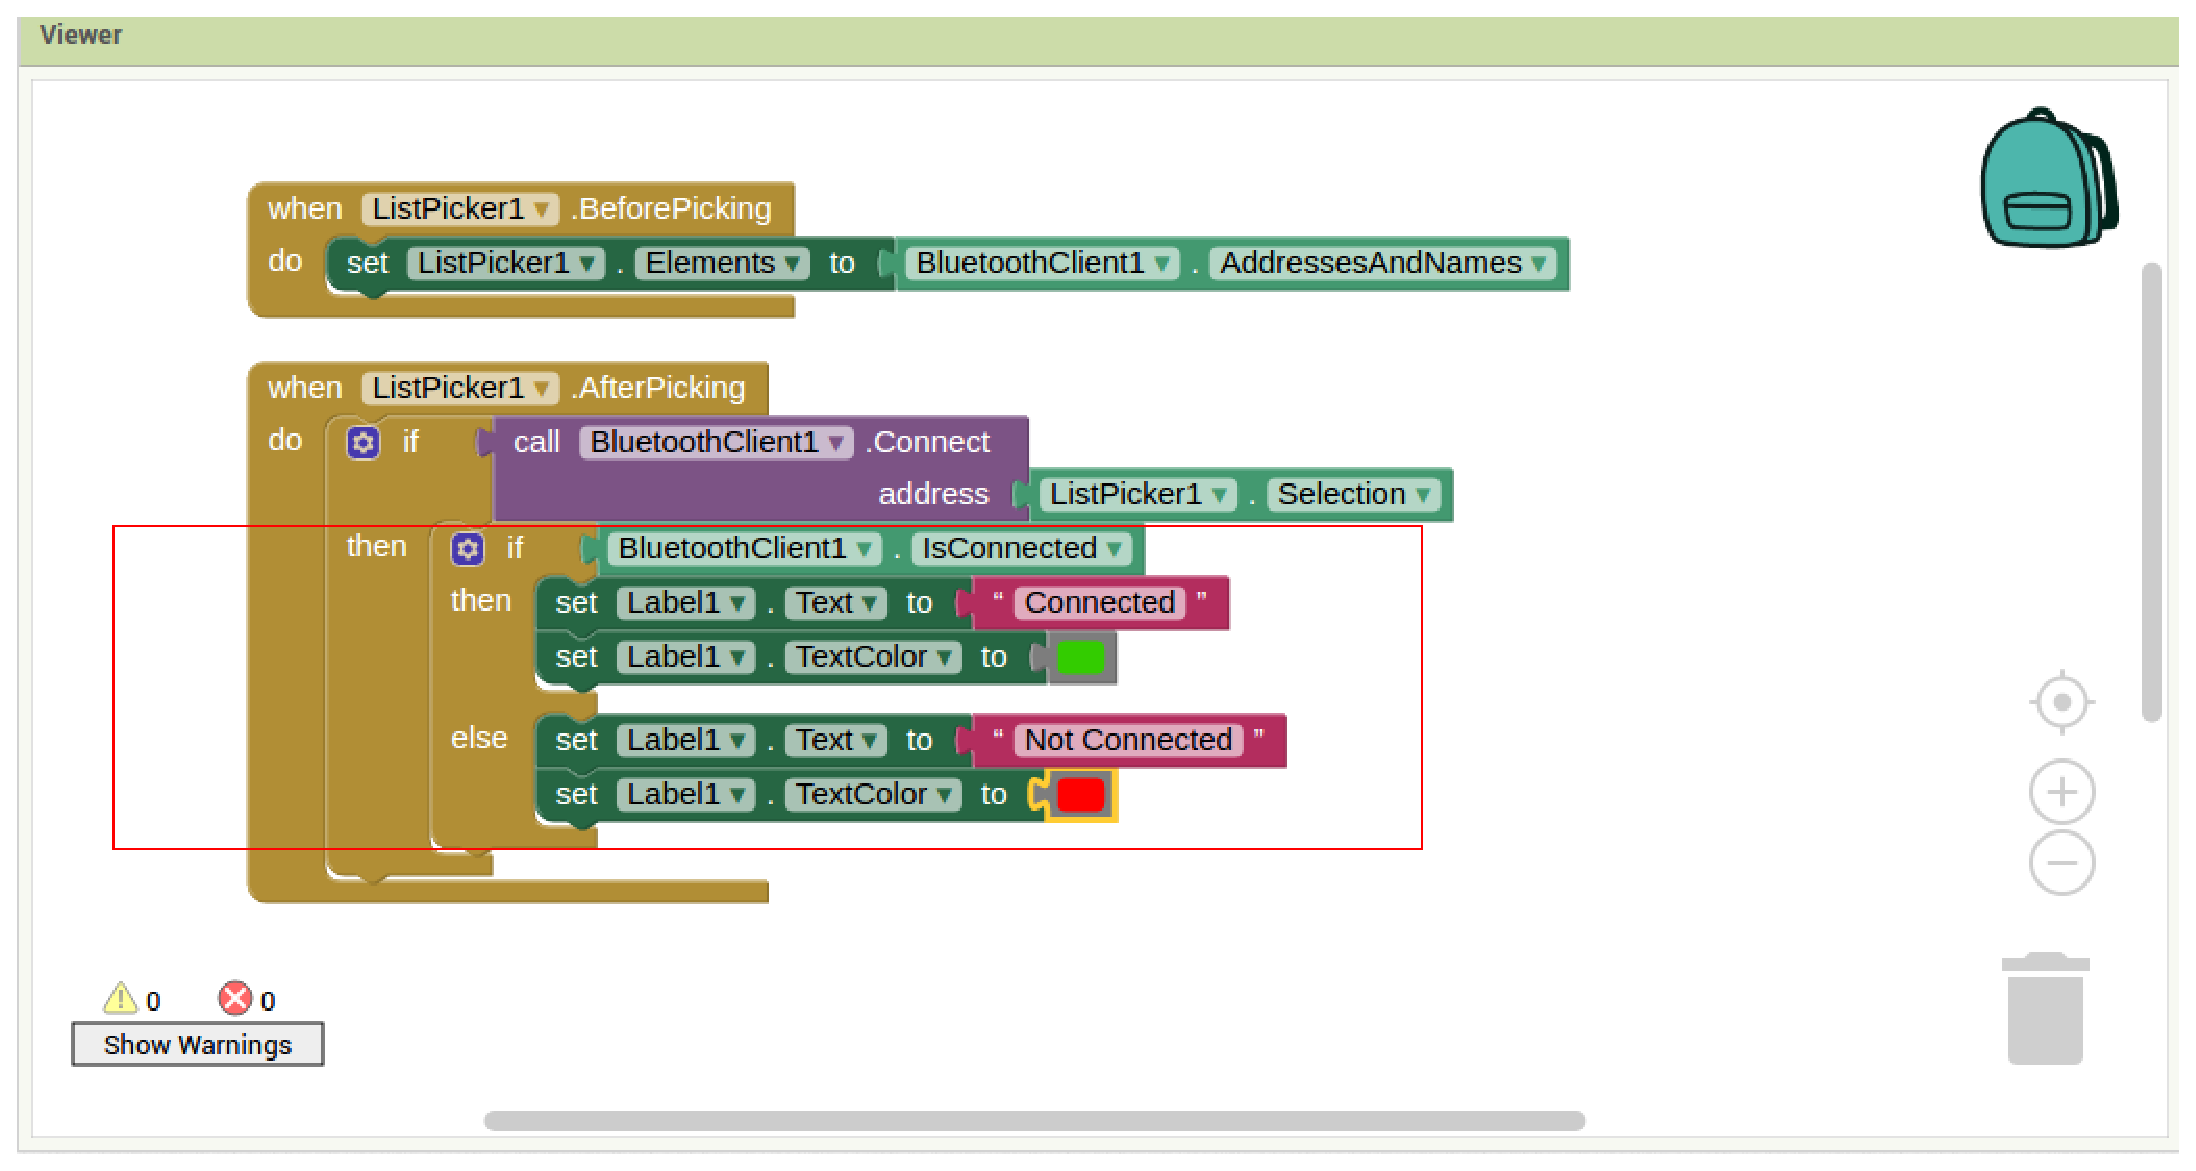
\includegraphics[width=\columnwidth]{./figs/11.png.eps}
\\
The group of components, highlighted within the red rectangular frame, is part of an event handler to change the status that either Bluetooth device is connected or not.
\begin{problem}
Continue and add the ``when Clock1.Timer" component from the Screen1$\backslash$Clock1 component group to the Viewer section. From the Built-in $\backslash$Control group, select and add the ``If then" component. Next, select and add the "BluetoothClient1.IsConnected" (from the Screen1$\backslash$BluetooothClient1 component group) and link to the ``if" condition and select ``set Label2.Text" (from the Screen1$\backslash$Label2 component group) component and link to the ``then" condition. Select and add the ``call BluetoothClient1.ReceiveTextnumberOfBytes" and ``call BluetoothClient1.BytesAvailabelToReceive" (from the Screen1$\backslash$BluetooothClient1 component group) components. Link them to get the following image.
%
\end{problem}
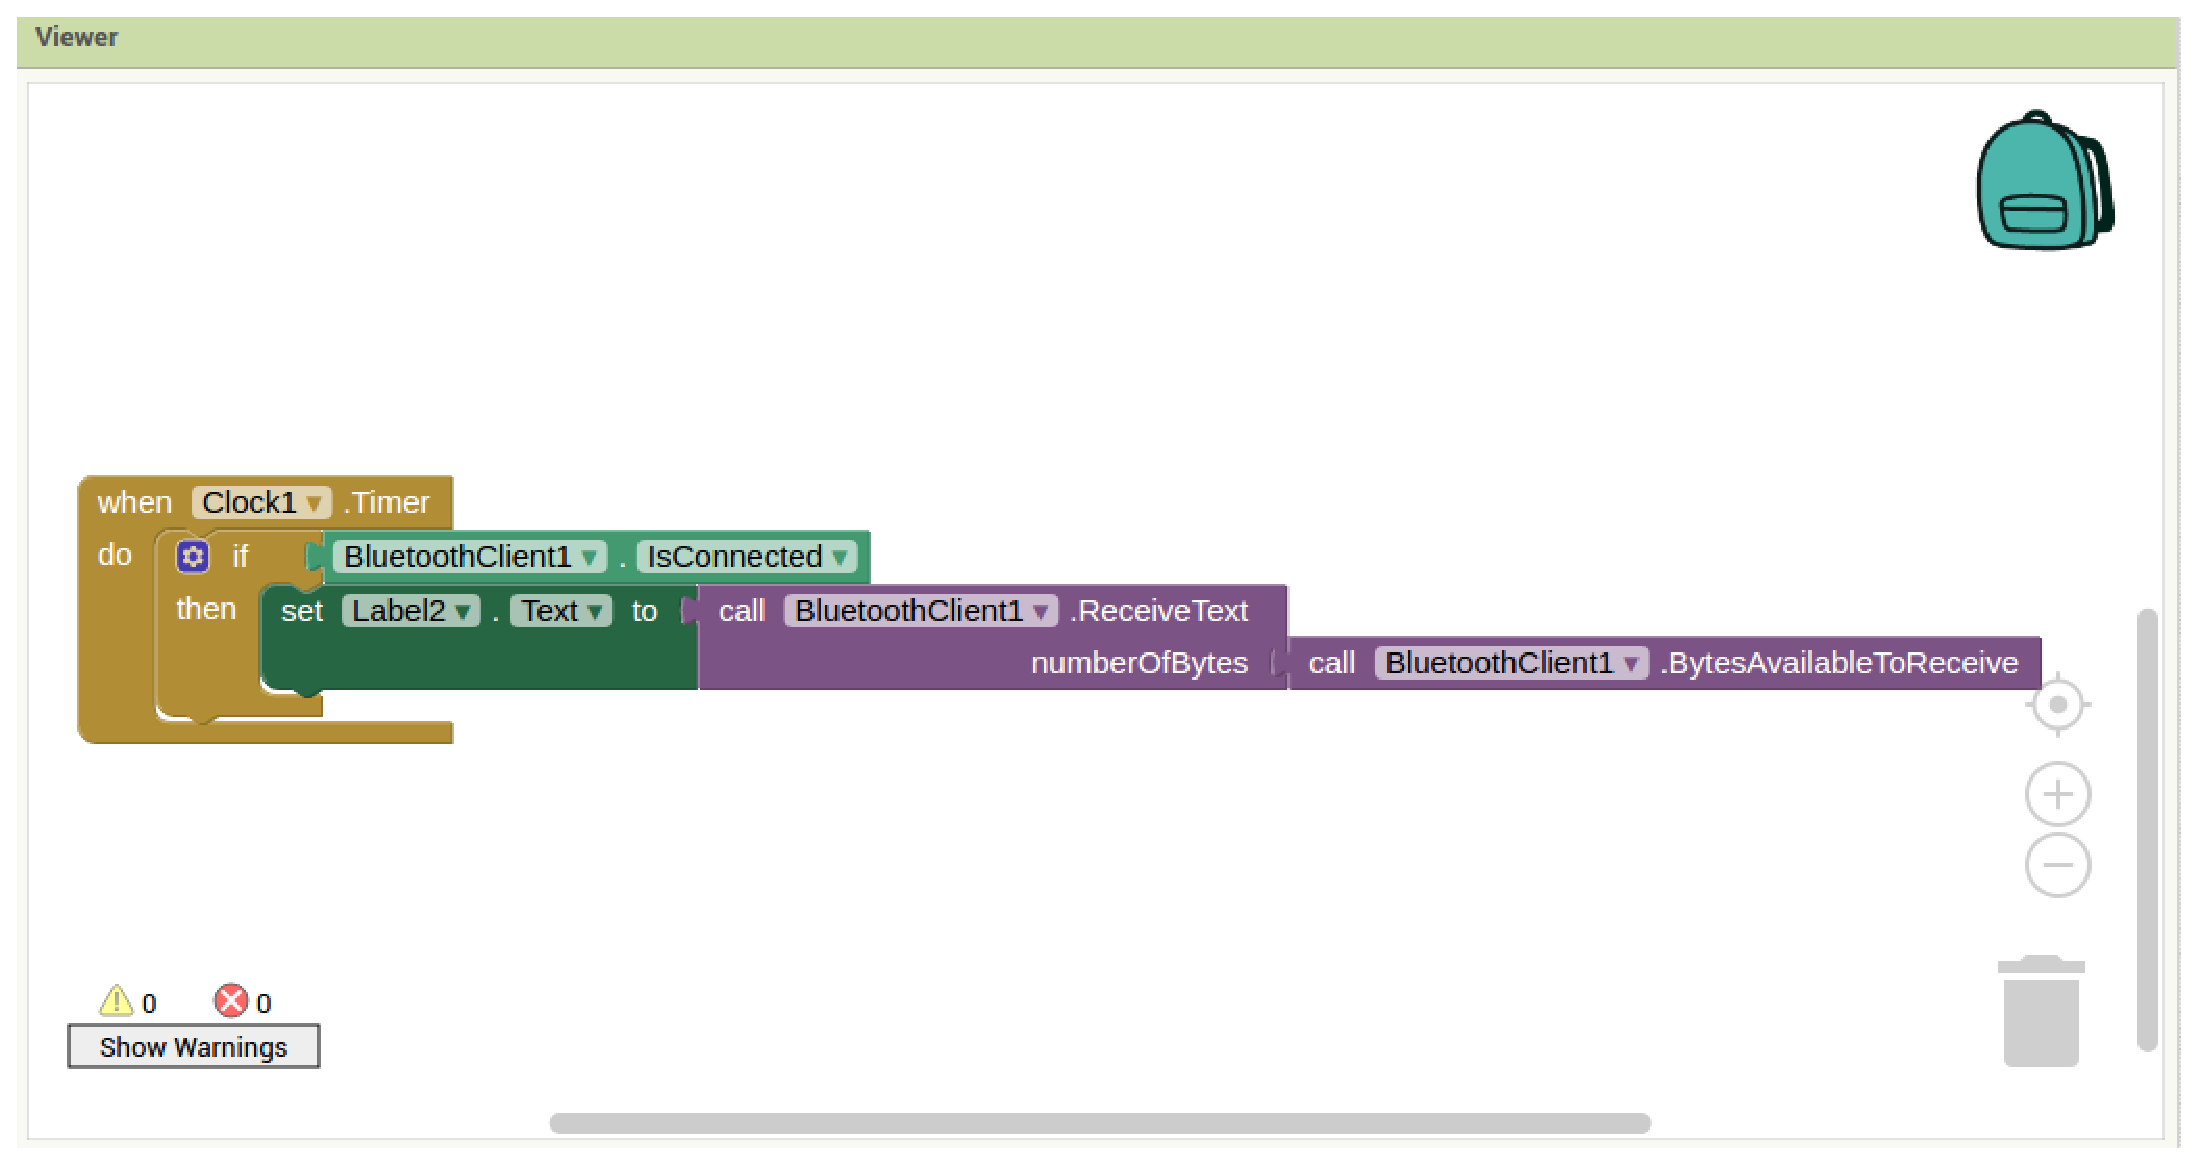
\includegraphics[width=\columnwidth]{./figs/12.png.eps}
\\
The above group of function block provide the program logic to display the measured resistance value, via the BluetoothClient1 connection to the connected Bluetooth device.
\begin{problem}
At this point, we have all of the intended function for the app. Before testing the app, we need to establish connectivity to a device or an emulator. To use a real device, you need to install the \textcolor{red}{MIT AI2 Companion} app from the \textcolor{blue}{App Store}. Install and launch the app on the target device.  After the MIT AI2 Companion app is launched, you have the option to enter a six digit code or use the scan QR code option to connect to App Inventor
\end{problem}
\includegraphics[width=\columnwidth]{./figs/5.png.eps}
\begin{problem}
From the App Inventor's \textcolor{blue}{Connect} menu, click on AI Companion to bring up the following screen and wait. Make sure that your computer and mobile device are connected to the same WiFi network.
\end{problem}
%
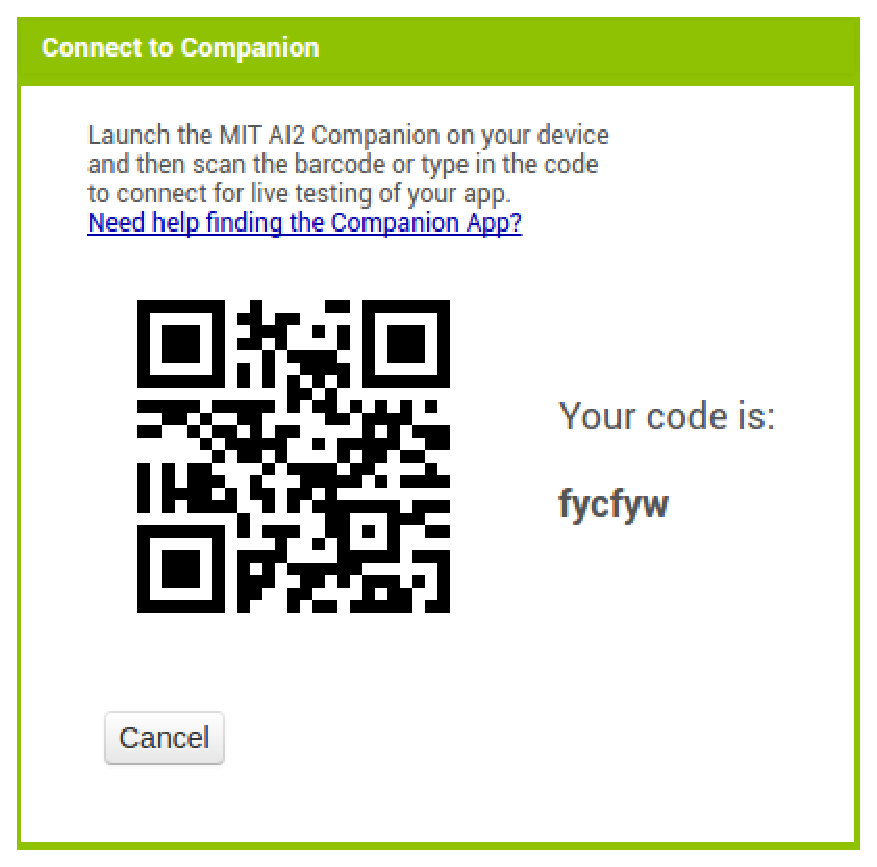
\includegraphics[width=\columnwidth]{./figs/13.png.eps}
%
\begin{problem}
From the target device, you can enter the six digit code, or scan the QR
code to establish connectivity to the App Inventor. Once connected, the app will display on the device, as shown below.  Note that this does not install the app on your device.
\end{problem}
\includegraphics[width=\columnwidth]{./figs/6.png.eps}
%
\begin{problem}
From the App Inventor \textcolor{blue}{Build} menu, click on \textcolor{red}{App(provide QR code for .apk)} to build the app. App Inventor shows the following progress as it builds the app
\end{problem}
\includegraphics[width=\columnwidth]{./figs/15.png.eps}
\begin{problem}
After the build is done, a QR code is provided for the MIT AI2 Companion to install the app, as shown below 
\end{problem}
%
\includegraphics[width=\columnwidth]{./figs/16.png.eps}
%
\begin{problem}
After scanning the QR code using MIT AI2 Companion, the following screen is shown on the device, asking for permission to install the app
\end{problem}
\includegraphics[width=\columnwidth]{./figs/14.png.eps}\\
%
Now install and launch the app on the device.
%
\section{Displaying Measured Resistance on Android App via Bluetooth}
Power off the Arduino.
\begin{problem}
Connect the TX pin of the Arduino to $R_2$.
\end{problem}
\begin{problem}
Connect the other end of $R_2$ to $R_1$
\end{problem}
\begin{problem}
Connect the other end of $R_1$ to GND.
\end{problem}
%
\begin{problem}
Connect A0 to RX pin of the Bluetooth module.
\end{problem}
%
\begin{problem}
Connect TX of Bluetooth to RX of Arduino.
\end{problem}
%
\begin{problem}
Make the $V_cc$ and GND connections for the Bluetooth module.  The final connection digram is available below.
\end{problem}
%
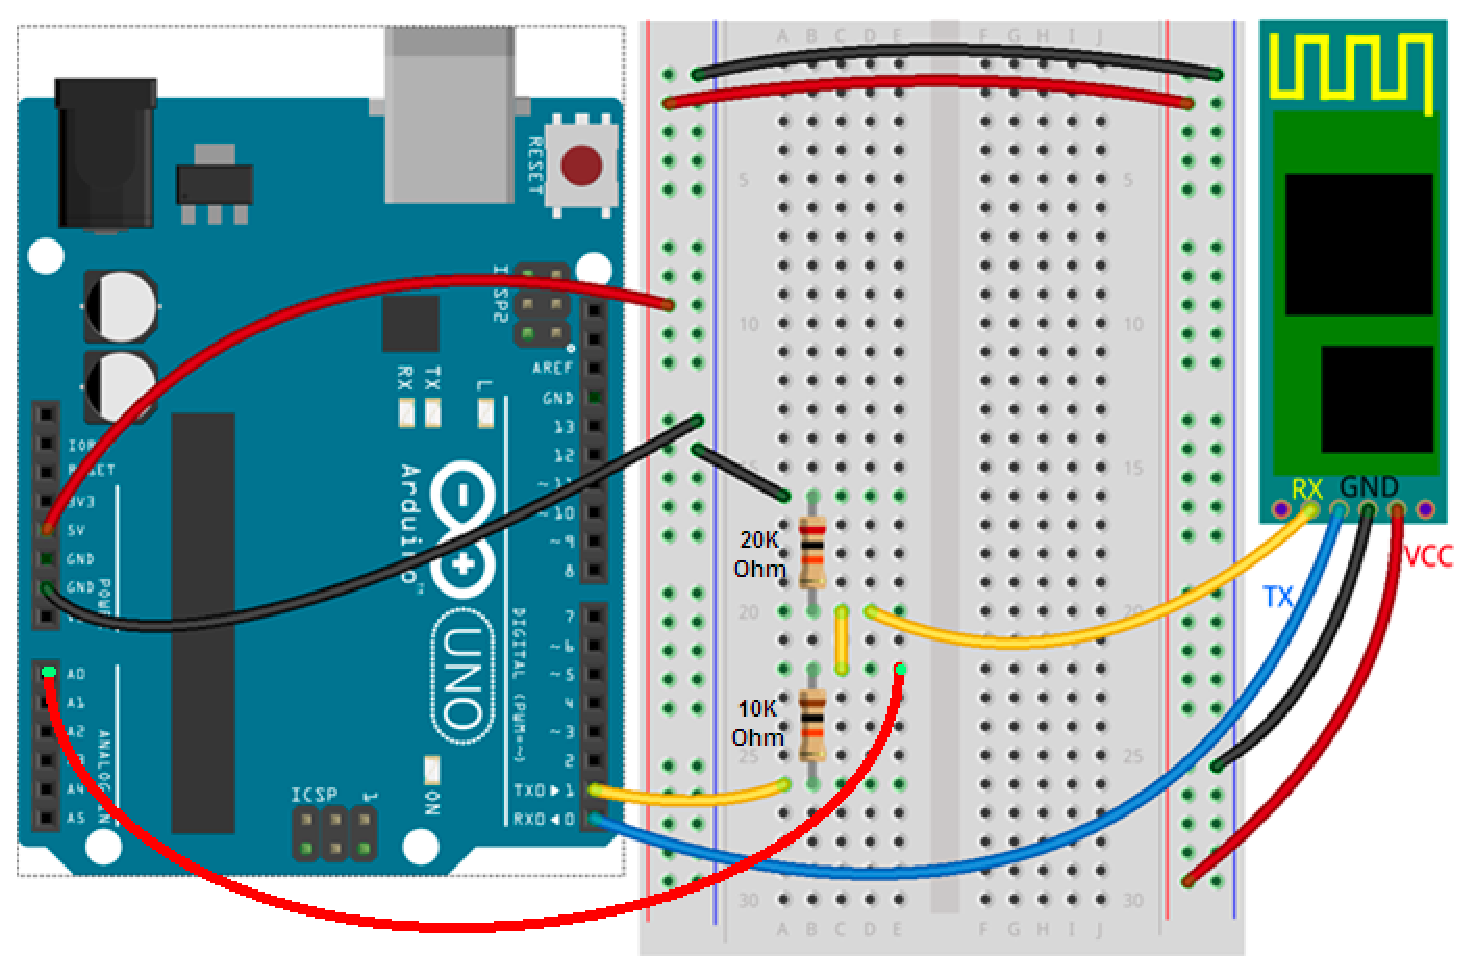
\includegraphics[width=\columnwidth]{./figs/Bluetooth-Module-Arduino-Uno.eps}
\begin{problem}
Power up the Arduino and get the code in Section I running.  Connect to the the bluetooth module and you should be able to see the resistance value on the app developed using the app inventor.
\end{problem}
%\solution 
%%
%\lstinputlisting{./codes/lcd/resistance_lcd.ino}
\section{Explanation}



\begin{enumerate}


\item We create a variable called analogPin and assign it to 0. 
This is because the voltage value we are going to read is connected to analogPin A0.



\item  The 10-bit ADC can differentiate 1024 discrete voltage levels, 5 volt is applied to 2 resistors and the voltage sample is taken in between the resistors. The value which we get from analogPin can be between 0 and 1023. 0 would represent 0 volts falls across the unknown resistor. A value of 1023 would mean that practically all 5 volts falls across the unknown resistor.



\item  $V_{out}$ represents the divided voltage that falls across the unknown resistor.



\item  The Ohm meter in this manual works on the principle of the voltage divider shown in Fig. \ref{fig:voltage_divider}.
%
\begin{align}
V_{out}&=\frac{R_1}{R_1+R_2}V_{in} \\
\Rightarrow R_2&=R_1\brak{\frac{V_{in}}{V_{out}}-1}
\end{align}
%
In the above, $V_{in} = 5$V, $R_1 = 220 \Omega$.
\end{enumerate}


\end{document}


